\documentclass[authordate, empirical]{jote-new-article}

\usepackage{caption}

\usepackage{tabularx}

\usepackage{graphicx}

\usepackage{hyperref}

\jotetitle{Attempt to identify Extracellular Vesicles derived from the Blood-Brain Barrier in peripheral blood}
\keywordsabstract{Blood-brain barrier, extracellular vesicles, flow cytometry, proteomics, psychosis}
\abstracttext{The blood-brain barrier (BBB) is hypothesized to play a role in the pathophysiology of psychosis. However, studying this structure in living humans is challenging due to limitations in current methods that fail to identify subtle changes or dysfunctions. Moreover, obtaining a biopsy is too invasive. To address these challenges, we aimed to isolate BBB-derived extracellular vesicles as potential biomarkers for neuropsychiatric conditions, providing a “liquid biopsy of the BBB”. Individuals with psychosis and healthy controls were recruited for this study. In the absence of single specific proteins for brain endothelial cells, we targeted three distinct proteins for immunolabelling. Proteomics and flow cytometry confirmed the presence of EV with the signature CD45-/CD31+/GLUT1+. Our efforts to generate adequate material for confirming proteomic analysis of EV with this signature were terminated due to excessive time and resource demands. This setback led us to recognize that our current approach was not feasible due to low abundance of EVs with the target signature. Moreover, the relative abundance of putative blood-derived EVs in comparison to putative (BEC)-derived EVs contradicted previously published data, raising concerns about the specificity of our approach.}
\runningauthor{Tunset et al.}
\jname{Journal of Trial \& Error}
\jyear{2025}
\paperdoi{10.36850/3738-4936}
\paperreceived{July 13, 2024}
\author[1]{\mbox{Mette Elise Tunset\orcid{0000-0001-7846-7629}}}
\affil[1]{St Olav's University Hospital}
\corremail{\href{mailto:mette.elise.tunset@stolav.no}{mette.elise.tunset@stolav.no}}
\corraddress{St Olav's University Hospital, Trondheim, Norway}
\runningauthor{Tunset \& Haslene-Hox}
\author[2]{\mbox{Hanne Haslene-Hox\orcid{0000-0001-7298-7332}}}
\affil[2]{Department of Biotechnology and Nanomedicine, Trondheim, Norway}
\paperaccepted{July 25, 2025}
\paperpublished{September 27, 2025}
\paperpublisheddate{2025-09-27}
\jwebsite{https://journal.trialanderror.org}

\begin{document}
\begin{frontmatter}
  \maketitle
  \begin{abstract}
    \printabstracttext
  \end{abstract}
\end{frontmatter}








	\section{Purpose}



	The blood-brain barrier (BBB) is hypothesized to play a role in the pathophysiology of psychosis. However, studying this structure in living humans is challenging due to limitations in current methods that fail to identify subtle changes or dysfunctions. We aimed to develop a method to isolate extracellular vesicles (EVs) in peripheral blood derived from the blood-brain barrier (BBB), offering a “liquid biopsy of the BBB”. We proposed that analyzing the content of these EVs would provide novel insights into BBB activity and signaling in humans, and launch potential biomarkers for neuropsychiatric conditions.








	\section{Introduction}



	The blood brain barrier (BBB) is crucial to maintain homeostasis and normal brain function (Kealy et al., 2020). BBB dysfunction has been proposed as a contributing factor in the pathophysiology of psychotic disorders (Kealy et al., 2020) and may represent a point of convergence between two leading hypotheses in schizophrenia research: elevated presynaptic dopamine synthesis (McCutcheon et al., 2020) and neuroinflammatory activation (Nayak et al., 2025).



	Experimental models have demonstrated that systemic inflammation can impair BBB integrity, allowing peripheral cytokines and immune cells to infiltrate the brain parenchyma (Chen et al., 2021). In schizophrenia, such immune-mediated permeability may expose midbrain dopaminergic circuits to inflammatory signals that affect dopamine regulation. Supporting this, post-mortem studies have reported increased macrophage density in the substantia nigra and changed tyrosine hydroxylase mRNA expression (Mendez-Victoriano et al., 2024).



	Beyond direct effects on dopamine synthesis, BBB disruption may indirectly contribute to dopaminergic dysregulation by altering the balance of excitatory and inhibitory neurotransmission (Brocco et al., 2022; Nayak et al., 2025). Cytokine-mediated dysfunction of parvalbumin-positive GABAergic interneurons and modulation of NMDA receptor signaling in glutamatergic neurons could lead to disinhibition of dopamine-producing cells, further amplifying dopaminergic output (Brocco et al., 2022; McCutcheon et al., 2020; Nayak et al., 2025).



	\begin{takeHomeMessage}EVs with the signature CD45-/CD31+/GLUT1+ thought to be derived from brain endothelial cells (BEC) were detected and isolated from peripheral blood by immunolabeling and flow cytometry. However, the proportion of EVs with this signature was too low to confirm a BEC origin by proteomics. Moreover, the relative abundance of putative blood-derived EVs in comparison to putative BEC-derived EVs contradicted previously published data, raising concerns about the specificity of our approach.
	\end{takeHomeMessage}

	A more speculative mechanism involves ionic dysregulation. The BBB tightly regulates extracellular pH, calcium, and potassium concentrations (Liu et al., 2024). Disruption of these gradients could alter neuronal excitability (Liu et al., 2024). Although reduced brain pH has been observed in some post-mortem studies of schizophrenia, the findings remain indirect and may reflect broader metabolic alterations rather than a direct consequence of BBB dysfunction (Park et al., 2021).



	Taken together, although these mechanisms remain hypothetical and evidence is still emerging, they suggest that BBB dysfunction could contribute to a cascade of immune, molecular, and network changes relevant to the development of psychosis. Its precise role, whether causal or part of a broader set of interacting processes, remains unclear.



	Despite its theoretical relevance, the BBB is difficult to study in living humans (Pollak et al., 2018), and currently available methods are limited. A spinal puncture with calculations of albumin ratios (blood/spinal fluid) can give indications of a leaky BBB (Kealy et al., 2020). Imaging techniques such as dynamic contrast-enhanced MRI can provide information about the integrity of the BBB, and such techniques have been shown to detect large abnormalities as in stroke, multiple sclerosis and brain tumors (Raja et al., 2018). However, imaging techniques remain inadequate to reliably detect low levels of BBB integrity loss (Raja et al., 2018). In addition, the detection of intracerebral molecules such as S100β in peripheral blood have been used as a marker of BBB leakage, but the demonstration of a brain lymphatic system (the glymphatics) makes the assumption that such proteins can only exit the brain via BBB leakage invalid (Plog et al., 2015). Thus, there are currently no established methods to detect low-grade permeability loss or isolate biological material from the BBB in a non-invasive way.



	EVs are vacuoles [Attention to author: should this be vesicles?] with a double lipid layer shed from all types of cells, containing proteins, lipids, and nucleic acids. EV have an important role in intercellular communication, both locally and systemically, as they transfer their contents between cells and thereby affect the recipient cell's status (Robbins \& Morelli, 2014). The half-life of EVs in blood of humans is unknown. However, in mice it is about 5 minutes and in macaques about 40 minutes. Thus, if the half-life in humans is in the same range, one could expect this to be a biomarker ideally suited for real-time status assessment of the BBB (Driedonks et al., 2022). The content of EVs reflect the status of the cell they originate from; their proteins can be used to trace their parent cell (Gomes \& Witwer, 2022). However, sorting out subpopulations of specific EVs requires highly specific and abundant surface proteins that can be used as immunolabelling targets to separate EVs of interest from other EVs and other particles in the blood (Gomes \& Witwer, 2022).



	To separate target EVs from other EVs and non-EV particles present in blood, we aimed to use multiple markers for subpopulation isolation — a strategy that, to our knowledge, has not been reported previously. We have not identified any studies isolating BBB-derived EVs. Although several studies have attempted to isolate brain-derived EVs, most have relied on suboptimal protein markers (Tunset et al., 2025). Many of these markers either lack specificity for the desired EV population or are not appropriately localized to the vesicle membrane, limiting their utility (Tunset et al., 2025). Among the markers evaluated to date, GLAST appears to be one of the most promising candidates, offering high brain specificity and membrane localization (Tunset et al., 2025).







	The brain endothelial cells (BEC) in the BBB are the bridge between the brain and its surroundings. When stressed, either by inflammatory stimulants or mechanical stress alone, BEC increases the secretion of EVs to both the abluminal (brain) and luminal (blood) side of the cell (Andrews et al., 2016; Yamamoto et al., 2015). Furthermore, BEC EVs can modulate the status of brain cells such as pericytes and oligodendrocytes (Kurachi et al., 2016; Yamamoto et al., 2015), suggesting that BEC-derived EVs in blood can also reflect processes occurring in the brain.











	\section{Methods}



	\subsection{Participants}



	The study included 25 individuals (6 females; \emph{M}\textsubscript{age} = 33.1, \emph{SD }= 11.0 years) assessed during either a first episode of psychosis or an acute exacerbation of an existing psychotic disorder. Diagnoses were determined using ICD-10 research criteria. Exclusion criteria included affective psychoses, organic causes of psychosis, cardiovascular disease, neurological disorders, rheumatic or autoimmune diseases, cancer, and pregnancy.







	Blood samples were collected at two time points: during the acute phase (T1), and after clinical improvement (T2), as determined by the Clinical Global Impression--Improvement Scale (CGI-I; Guy, 1976). Follow-up samples were obtained from 18 participants (\emph{M}\textsubscript{sample} = 79, \emph{SD }= 34 days). Substance use was screened through self-report and urine drug testing at T1, and by self-report at T2.







	A control group of 25 age- and sex-matched individuals (\emph{M}\textsubscript{age} = 34.2, \emph{SD }= 11.2 years) was included. Controls were screened for the same exclusion criteria, including recent substance use.







	\subsection{Ethics}



	The study was approved by the Regional Ethics committee, South East Norway (2016/949). All participants gave written informed consent.







	\subsection{EV isolation}



	Peripheral blood was collected from patients and healthy controls in EDTA-treated tubes. Plasma was isolated by centrifugation at 2,000 g for 30 minutes at 4°C, followed by a second spin at 10,000 g for 30 minutes at 4°C. Pellets were stored at -80°C. For further processing, pellets were thawed, resuspended in PBS, pooled, and centrifuged again at 2,000 g for 30 minutes at 4°C to remove residual cells and large debris. The resulting supernatant was centrifuged at 10,000 g for 30 minutes at 4°C (Tunset et al., 2020; Tunset et al., 2023).







	\subsection{Isolation of EV with BEC origin }



	To separate EVs originating from endothelial cells of the BBB from other EVs present in peripheral blood, we need specific membrane protein markers to use as target for antibodies. However, no single protein is specific to BEC (Sjöstedt et al., 2015). To be able to specifically target the BEC-EVs we thus need to select EVs with a multi-protein identifying profile. In an adult, glucose transporter 1 (or GLUT1) is expressed at the highest levels in erythrocytes and in the endothelial cells of barrier tissues such as the blood--brain barrier, but is also expressed in white blood cells (Hussar et al., 2002; Maratou et al., 2007; Takata et al., 1993; Takata et al., 1997). Platelet endothelial cell adhesion molecule-1 (PECAM-1/CD31) is expressed on the surface of platelets and mononuclear blood cells, as well as in endothelial cell intercellular junctions, where it maintains endothelial integrity (Heddini et al., 2001; Newman, 1997). CD31 is not present on erythrocytes or epithelial cells. CD45 antigen (leukocyte common antigen) is expressed on almost all hematopoietic cells except for mature erythrocytes (Altin \& Sloan, 1997). CD45 is not expressed in endothelial cells.



	Thus, the EV fraction originating from the BEC should have a specific signature of CD45-/CD31+/GLUT1+. By employing specific antibodies for these membrane proteins, we can use a flow cytometer with cell sorting to isolate the EV fraction with this specific signature. These markers would in theory also isolate circulating cells with the same proteins, but whole cells are excluded by the initial centrifugation and will not be present in the EV fractions. Although cells with this signature used in this experiment have been isolated, they were not assessed to verify BEC origin (Pourcyrous et al., 2015).



	Since there are no EV standards with known antibody status readily available, we used blood cells (positive controls for CD31 and CD45) and the cell line HepG2 (positive control for GLUT1) to optimize the antibody staining protocol and as positive controls in flow cytometry analyses. EVs isolated by centrifugation at 10,000g (10 µL) were diluted in PBS (1:10) with added antibodies (5µL) for CD45 (BUV805 Mouse Anti-Human CD45, BD Biosciences, Cat. No: 564914), CD31 (Alexa Fluor® 488 Mouse Anti-Human CD31, BD Biosciences, Cat. No. 558068), and GLUT1 (Alexa Fluor® 647 Anti-Glucose Transporter GLUT1 antibody [EPR3915] Abcam, Cat. No: ab195020) and incubated 1 hour for staining. Samples were further diluted 1:10 in sheet fluid and run by flow cytometry until 50,000 events were registered per sample (Beckman Coulter MoFlo Asterios). A repeated run was performed for two samples up to 2 million registered events (approximately 2 hours per sample), where the CD45-/CD31+/GLUT1+ and CD45+/CD31+/GLUT1+ fractions were isolated. The resulting fraction tubes were washed out with 100 µL PBS and the protein content of the resulting samples were measured by Qubit Fluorometer 4.0 (10-20 µL input sample for analysis). We used the following gating strategy: (a) removal of doublets, (b) selection of CD45-/CD31+ events from a dot-plot of the main population, and (c) using these events to select the CD45-/CD31+/GLUT1+ population on a histogram. Analysis was performed on FlowJo v10.10.0.







	\begin{figure}
		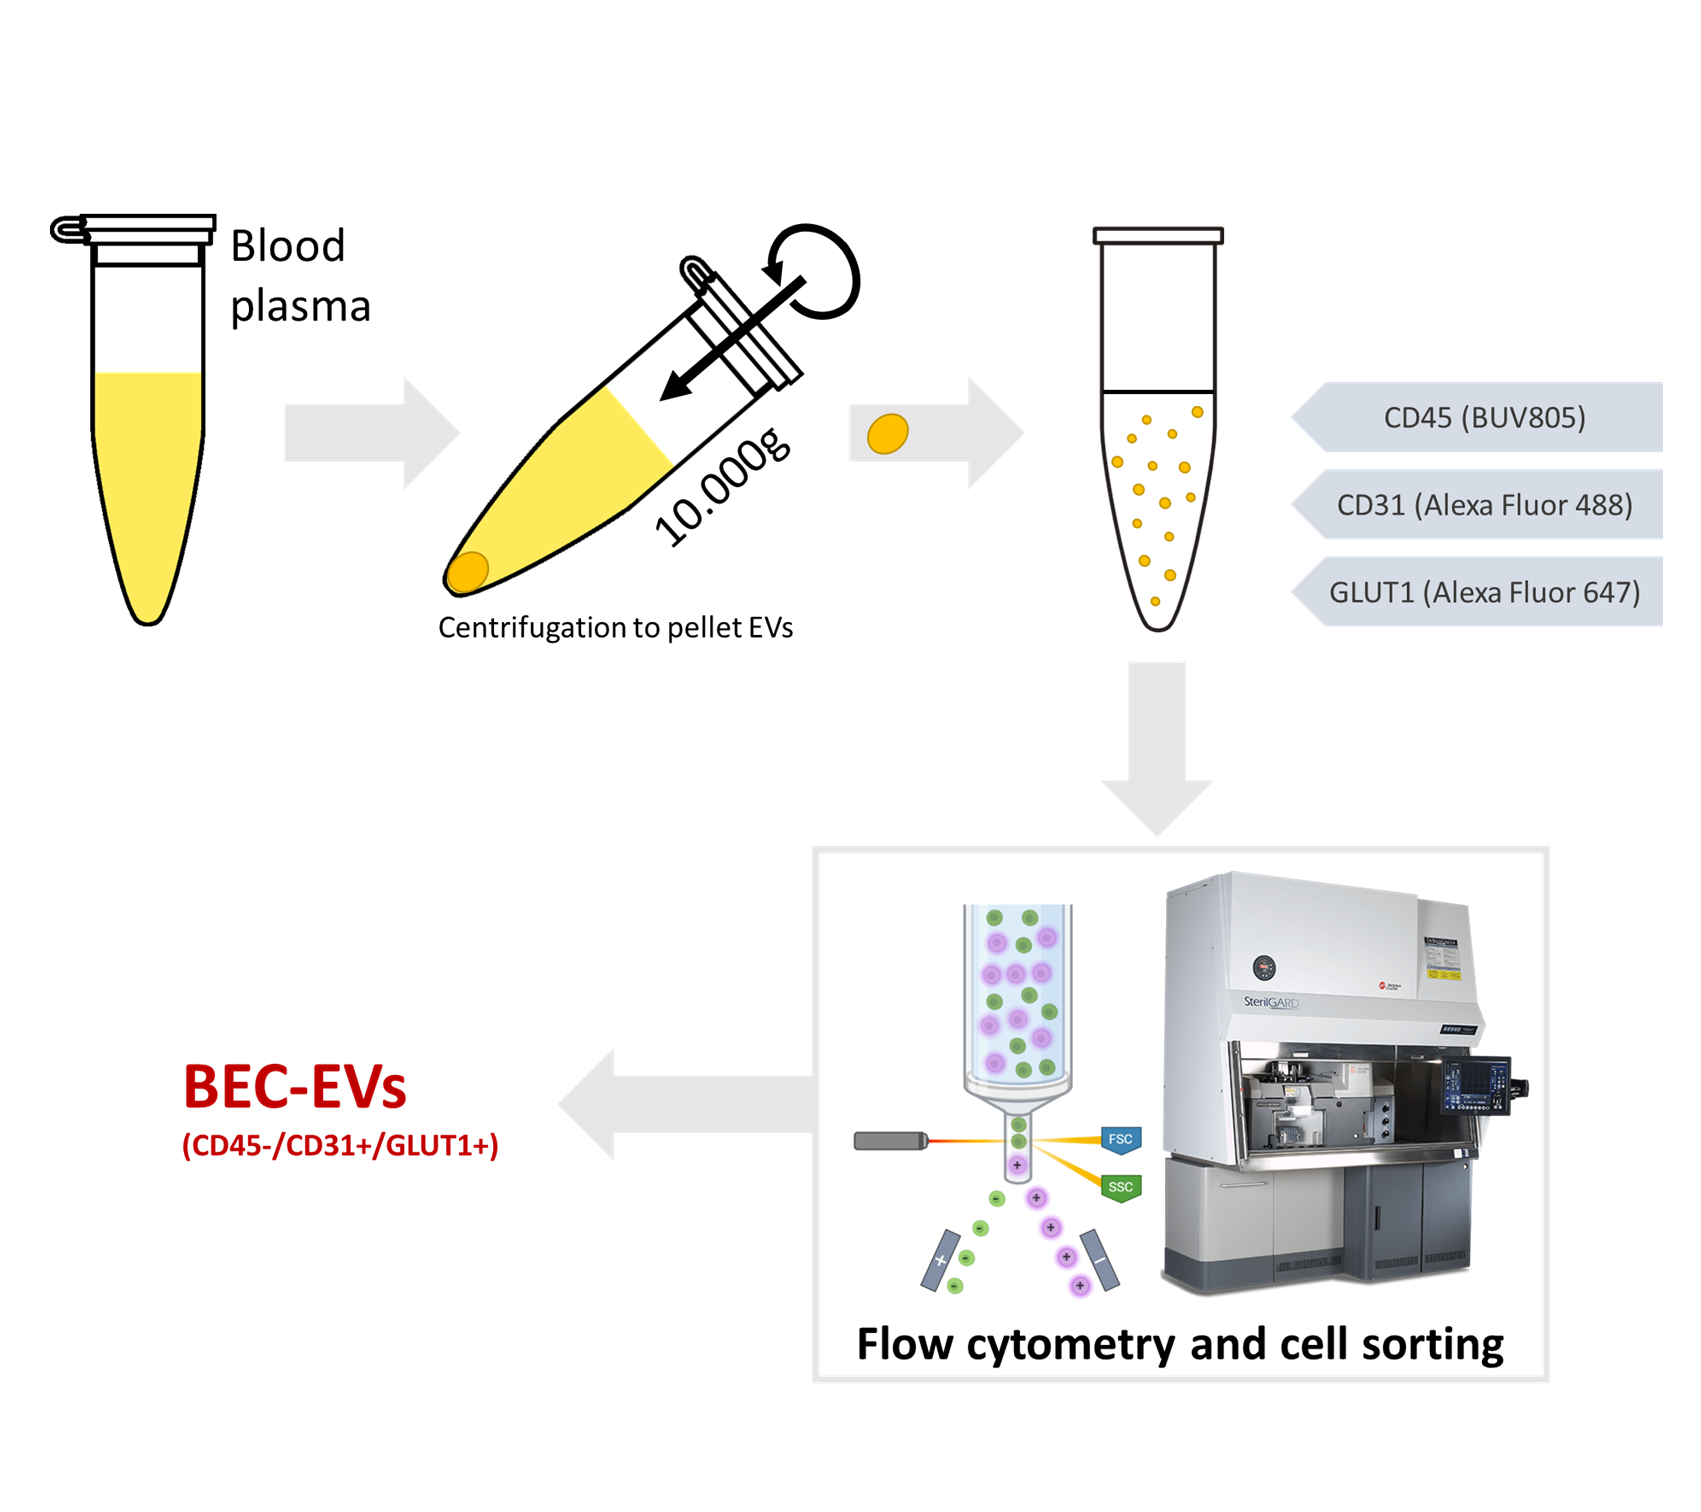
\includegraphics[width=\linewidth]{media/image1.png}

		\caption{Overview of the laboratory procedures planned in this study}

		\label{fig:rId8}


	\end{figure}



	



	\emph{ }



	\subsection{Proteomic analyses}



	We planned to perform proteomic analyses on both sorted and total EV fractions using high-resolution shotgun MS. This would provide a comprehensive list of proteins present in the samples as well as signal abundance and number of peptide-spectra matches for each protein. If isolation of BECs was successful, we expected to identify enrichment of brain- and BEC-specific proteins, which would have supported the BEC origin of the isolated EVs. As no protein is uniquely expressed in BECs, we intended to examine a panel of BEC-enriched proteins with varying expression across other tissues based on the human protein atlas (Sjöstedt et al., 2020). A consistent increase in these proteins in the sorted EVs compared to total EVs would indicate selective enrichment of BEC-derived EVs. Examples are occludin (Rom et al., 2020), MCAM, and ABCB1 (Sjöstedt et al., 2020). Also, we planned to assess proteins that are not expressed in the BBB as a negative marker, such as BNIP5 and ApoA4 (Sjöstedt et al., 2020). In addition, comparing the proteomic findings from healthy and psychotic patients could potentially identify altered content and thereby functional characteristics of the originating cells.



	\section{Results}



	Initial proteomics analysis confirmed the presence of EV markers as well as the proteins used for immunolabelling within the total EV fraction (Tunset et al., 2020). Thus, flow cytometry was performed with the selected antibody signatures. However, the presence of the expected BEC signature was significantly decreased in psychotic patients compared with healthy controls, in contrary to the initial hypothesis (Figure 2). Nevertheless, we attempted sorting on the antibody signature evaluate feasibility of the approach. After an extended period of sorting (\textasciitilde{}2h, 2 x 10\textsuperscript{6} sorted events), the resulting protein content in sorted samples was miniscule (1.5-3 µg of total protein), below the required protein amounts for further sample handling and in-depth proteomic analyses.



	\begin{figure}
		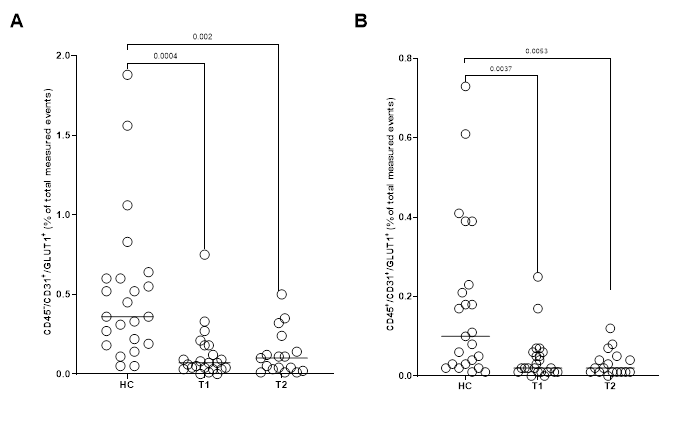
\includegraphics[width=\linewidth]{media/image2.png}

		\caption{Flow cytometry data of EVs from patients with psychotic disorders at the acute state of psychosis (T1), after improvement (T2) and healthy controls (HC). A) Frequency of events with a signature CD45-/CD31+/GLUT1+ hypothesized to be derived from BBB endothelial cells and B) Frequency of events with a signature of CD45+/CD31+/GLUT1+ expected to be derived from white blood cells. Significance determined by two-tailed unpaired Student's t-test.}

		\label{fig:rId9}


	\end{figure}














	\section{Discussion}



	Our chosen isolation method produced EV populations with the highest concentrations falling within the 100-200 nm size range (Tunset et al., 2020), and we obtained good detection of EVs of this size with the Beckman Coulter MoFlo Asterios high-velocity cell sorter used in our experiments.



	The flow cytometry confirmed that EVs with the profile CD45-/CD31+/GLUT1+ were present in the blood of healthy controls and patients with psychotic disorders, although they were more prevalent in healthy controls, contradictory to our hypothesis. There were also significant differences between groups in CD45+/CD31+/GLUT1+ EVs, thought to be derived from white blood cells (decreased in patients).



	We detected approximately four times more EVs hypothesized to originate from BECs than from the population expected to originate from white blood cells. This raised concerns about the validity of our findings, as EVs in blood are predominantly derived from blood cells, with only a smaller fraction originating from endothelial cells (Nieuwland \& Siljander, 2024). Since we were attempting to isolate a subfraction of endothelial-derived EVs, this result is particularly incongruent.



	Between 60\% and 99\% of the single EVs measured by flow cytometry were negative for both CD45 and CD31. This is in contradiction to a study by Li et al. (2020) analyzing RNA content from 101 human plasma samples which found that 99.8\% of circulating EVs originate from hematopoietic cells, with 51\% being platelet-derived. Notably, EVs with the CD45+/CD31+/GLUT1- signature, which would be expected from white blood cells, accounted for only 0--6.8\% of events in our experiment, compared to approximately 45\% in the Li et al. study. This discrepancy may reflect several factors, including the lack of direct correlation between surface protein markers and RNA cargo, as well as methodological differences in EV isolation and sampling, which could lead to enrichment of different EV subpopulations.







	Detecting EV with the signature CD45-/CD31+/GLUT1+ by flow cytometry with 10,000 to 50,000 events takes minutes. However, the isolation by flow sorting of these EVs in the abundances required for further analyses necessitated millions of sorted events, requiring several hours to process a single sample. The chosen EV isolation method yielded a mean EV concentration of 2.4x10\textsuperscript{7} (SD 1,1x10\textsuperscript{7}) EV/mL plasma in patients and 1.2x10\textsuperscript{7} (SD 5.0x10\textsuperscript{6}) EV/mL plasma in healthy controls (Tunset et al., 2020). Although our yield was low, the fluid prepared for cytometry had a mean concentration of 1.29x10\textsuperscript{9} EV/ml, which is suitable for flow cytometry (Welsh et al., 2020). Our low yield meant that we had limited material for method optimization and further testing, although this was not our primary challenge. 



	We concluded that our current approach had both specificity and feasibility issues. The challenges may stem from our selection of proteins: Even with good parent cell characterization, the EVs may not have the same density of target proteins, making the target proteins unsuitable for specific EV sorting. As an example, many studies have used L1CAM as a capture protein for "neuroEV" isolated from peripheral blood in psychiatric research (Goetzl et al., 2021; Lee et al., 2021; Nasca et al., 2020; Mansur et al., 2020; Mansur et al., 2021; Saeedi et al., 2021; Singh et al., 2023; Qin et al., 2022). However, there are specificity issues (Sjöstedt et al., 2020) and evidence indicates that L1CAM is not expressed in EVs derived from blood and cerebrospinal fluid (Norman et al., 2021). At present, GLAST appears to be one of the most promising markers for studying brain-derived EVs (Tunset et al., 2025).



	Furthermore, aggregation of EVs could mask the protein signature of individual EVs, altering the overall populations in a non-systematic manner, and likely increasing the presence of populations positive for multiple markers. EV aggregation can be an artifact arising from e.g., what anti-coagulant is used, freeze-thaw cycling, or the presence of platelets (Ahmadian et al., 2024). For further studies, researchers should consider using citrate as an anti-coagulant and restricting the number of freeze-thaw cycles to a minimum. Although citrate is often regarded as a better choice for preserving EV integrity, evidence remains inconsistent, with some studies suggesting that EDTA outperforms citrate in stabilizing EVs (Buntsma et al., 2022). Aggregates could also be specifically removed by differential (density gradient) centrifugation or “restrict size” in flow cytometry and cell sorting.



	In addition, the flow cytometry sorting approach is further hampered by small amounts of material and the absence of positive EV controls that could be used to optimize event selection with a specific antibody in flow cytometry analysis. Stringent gating of size and antibody intensity are needed during flow cytometry analysis to be able to select small populations. To correctly define data filters, antibody controls should ideally be both the same size and type, and should have a verified presence of the target antigens. At present, this is not typically available for EVs. Purification methods other than flow cytometry (e.g., immune precipitation with magnetic beads) could be considered to increase the throughput of the isolation method, while flow cytometry can act as a good verification of the prevalence of an interesting population.



	Another possible explanation for the observed specificity issues is the recently discovered EV corona — a layer of biomolecules that naturally adhere to the EV surface in biological fluids like blood (Toth et al., 2021). If proteins from the surrounding fluid bind to EVs, they could obscure the original protein profile, leading to a more uniform signature across different EV populations. Thus, the presence of the corona would raise critical concerns for the liquid biopsy approach. However, the unexpectedly low proportion of EVs with white blood cell signatures suggests that the corona did not influence our results. If the corona had done so, we would have expected a higher proportion of EVs with positive signature as in the white blood cell population and a much lower proportion in the signature demanding the absence of a common protein. Our findings therefore support the notion that the EV corona is not a major confounding factor when sorting EVs using immunolabeling.







	We conclude that isolating EV based on antibody signals with flow cytometry is possible and can provide relevant information on its own. However, yield becomes important for further analyses: You must have enough EV starting material. Our example, isolating 1-3 µg of protein from 2 million events on a cell sorter, is a relevant metric to consider for similar experimental setups. Such an amount may be enough for sensitive proteomic analyses, but it is also important to consider the extensive sample preparation with the inherent risk of reduced yield, and, with small amounts of material, the risk of absorbance to labware during sample handling.



	Given the challenges with specificity and yield, we decided not to pursue the isolation of BEC EVs by modifying aspects of the project, such as the immunomarkers. This decision was based on the requirement of large EV samples [Attention to authors: What do you mean to say? Is there a large / important need /requirement for samples, or are the samples themselves supposed to be large in size?] for method optimization, the excessive time required for such lab-intensive methods, and the low likelihood that such minor adjustments would lead to substantial improvements.



	To pursue the idea of isolating a liquid biopsy of the BBB, we recommend selecting an isolation method that provides a high yield of EVs, providing enough material for extensive testing. However, certain high-yield methods, such as polymer-based precipitation, pose significant contamination risks when applied to blood-derived samples (Veerman et al., 2021). Thus, care must be taken at all steps to minimize EV aggregation; from sample collection (selection of anticoagulant), freezing and thawing, to EV isolation (Bettio et al., 2023). For antibody-based methods, it is essential to optimize antibody binding using biologically relevant EV material to confirm that the target surface proteins are indeed present and expressed at a sufficient density to allow reliable detection and sorting. EVs isolated from cell culture may serve as a well-characterized and consistent standard to support antibody optimization and protocol standardization, particularly for flow cytometry.



	Techniques from the field of single-cell proteomics (Gatto et al., 2023), where very small protein amounts are used for proteomic profiling, could facilitate the confirmation of proteomics in very small volumes of EV. This would circumvent the issues of low protein output, or make EV population analysis possible with other methods than flow cytometry (e.g., based on single-cell methodologies).











	\section{Conclusion }



	While our study detected EVs with the surface marker profile CD45-/CD31+/GLUT1+ in peripheral blood, the proportions of the signatures raised concerns about their specificity for BEC. Moreover, the low yield of sorted EVs rendered downstream proteomic analysis unfeasible, highlighting a limitation in scalability. These results underscore the technical and biological challenges of isolating sub-populations of EVs from blood using current antibody-based approaches with further downstream applications in mind. We further raise the need for better EV-specific standards to be developed, which will counter some of the challenges in EV-flow cytometry. We emphasize that a reliable “liquid biopsy” of the BBB will require not only well-validated surface markers but also optimized EV isolation protocols that preserve epitope accessibility and deliver sufficient material for characterization. Although there are technical challenges to using EVs to access BBB-related biological material, further research is needed to investigate how EVs can inform our understanding of BBB function in the context of psychosis. Such studies may offer valuable insights into disease mechanisms and support the development of novel therapeutic strategies.







	\section{References}



	Ahmadian, S., Jafari, N., Tamadon, A., Ghaffarzadeh, A., Rahbarghazi, R., \& Mahdipour, M. (2024). Different storage and freezing protocols for extracellular vesicles: A systematic review. \emph{Stem Cell Research \& Therapy},\emph{ 15}(1), Article 453. \url{https://doi.org/10.1186/s13287-024-04005-7}



	Altin, J. G., \& Sloan, E. K. (1997). The role of CD45 and CD45-associated molecules in T cell activation. \emph{Immunology \& Cell Biology},\emph{ 75}(5), 430-445. \url{https://doi.org/10.1038/icb.1997.68}



	Andrews, A. M., Lutton, E. M., Merkel, S. F., Razmpour, R., \& Ramirez, S. H. (2016). Mechanical injury induces brain endothelial-derived microvesicle release: Implications for cerebral vascular injury during traumatic brain injury. \emph{Frontiers in Cellular Neuroscience},\emph{ 10}, Article 43. \url{https://doi.org/10.3389/fncel.2016.00043}



	Bettio, V., Mazzucco, E., Antona, A., Cracas, S., Varalda, M., Venetucci, J., Bruno, S., Chiabotto, G., Venegoni, C., Vasile, A., Chiocchetti, A., Quaglia, M., Camussi, G., Cantaluppi, V., Panella, M., Rolla, R., Manfredi, M., \& Capello, D. (2023). Extracellular vesicles from human plasma for biomarkers discovery: Impact of anticoagulants and isolation techniques. \emph{PloS One},\emph{ 18}(5), Article e0285440. \url{https://doi.org/10.1371/journal.pone.0285440}



	Brocco, D., De Bellis, D., Di Marino, P., Simeone, P., Grassadonia, A., De Tursi, M., Grottola, T., Di Mola, F. F., Di Gregorio, P., Zappacosta, B., Angelone, A., Lellis, L., Veschi, S., Florio, R., De Fabritiis, S., Verginelli, F., Marchisio, M., Caporale, M., Luisi, D., ... Lanuti, P. (2022). High blood concentration of leukocyte-derived extracellular vesicles is predictive of favorable clinical outcomes in patients with pancreatic cancer: Results from a multicenter prospective study. \emph{Cancers},\emph{ 14}(19), Article 4748. \url{https://doi.org/10.3390/cancers14194748}



	Buntsma, N. C., Gasecka, A., Roos, Y., van Leeuwen, T. G., van der Pol, E., \& Nieuwland, R. (2022). EDTA stabilizes the concentration of platelet-derived extracellular vesicles during blood collection and handling. \emph{Platelets},\emph{ 33}(5), 764-771. \url{https://doi.org/10.1080/09537104.2021.1991569}



	Chen, F., Zou, L., Dai, Y., Sun, J., Chen, C., Zhang, Y., Peng, Q., Zhang, Z., Xie, Z., Wu, H., Tian, W., Yu, X., Yu, J., \& Wang, K. (2021). Prognostic plasma exosomal microRNA biomarkers in patients with substance use disorders presenting comorbid with anxiety and depression. \emph{Scientific Reports},\emph{ 11}(1), Article 6271. \url{https://doi.org/10.1038/s41598-021-84501-5}



	Driedonks, T., Jiang, L., Carlson, B., Han, Z., Liu, G., Queen, S. E., Shirk, E. N., Gololobova, O., Liao, Z., Nyberg, L. H., Lima, G., Paniushkina, L., Garcia-Contreras, M., Schonvisky, K., Castell, N., Stover, M., Guerrero-Martin, S., Richardson, R., Smith, B., ... Witwer, K. W. (2022). Pharmacokinetics and biodistribution of extracellular vesicles administered intravenously and intranasally to Macaca nemestrina. \emph{Journal of Extracellular Biology},\emph{ 1}(10), Article e59. \url{https://doi.org/https://doi.org/10.1002/jex2.59}



	Gatto, L., Aebersold, R., Cox, J., Demichev, V., Derks, J., Emmott, E., Franks, A. M., Ivanov, A. R., Kelly, R. T., Khoury, L., Leduc, A., MacCoss, M. J., Nemes, P., Perlman, D. H., Petelski, A. A., Rose, C. M., Schoof, E. M., Van Eyk, J., Vanderaa, C., ... Slavov, N. (2023). Initial recommendations for performing, benchmarking and reporting single-cell proteomics experiments. \emph{Nature Methods},\emph{ 20}(3), 375-386. \url{https://doi.org/10.1038/s41592-023-01785-3}



	Goetzl, E. J., Wolkowitz, O. M., Srihari, V. H., Reus, V. I., Goetzl, L., Kapogiannis, D., Heninger, G. R., \& Mellon, S. H. (2021). Abnormal levels of mitochondrial proteins in plasma neuronal extracellular vesicles in major depressive disorder. \emph{Molecular Psychiatry},\emph{ 26}(12), 7355-7362. \url{https://doi.org/10.1038/s41380-021-01268-x}



	Gomes, D. E., \& Witwer, K. W. (2022). L1CAM-associated extracellular vesicles: A systematic review of nomenclature, sources, separation, and characterization. \emph{Journal of Extracellular Biology},\emph{ 1}(3), Article e35. \url{https://doi.org/10.1002/jex2.35}



	Guy, W. (1976). \emph{ECDEU Assessment Manual for Psychopharmacology. }National Institute of Mental Health (U.S.).



	Heddini, A., Chen, Q., Obiero, J., Kai, O., Fernandez, V., Marsh, K., Muller, W. A., \& Wahlgren, M. (2001). Binding of Plasmodium falciparum-infected erythrocytes to soluble platelet endothelial cell adhesion molecule-1 (PECAM-1/CD31): Frequent recognition by clinical isolates. \emph{American Journal of Tropical Medicine and Hygiene},\emph{ 65}(1), 47-51. \url{http://doi.org/10.4269/ajtmh.2001.65.47}



	Hussar, P., Tserentsoodol, N., Koyama, H., Yokoo-Sugawara, M., Matsuzaki, T., Takami, S., \& Takata, K. (2002). The glucose transporter GLUT1 and the tight junction protein occludin in nasal olfactory mucosa. \emph{Chemical Senses},\emph{ 27}(1), 7-11. \url{http://doi.org/10.1093/chemse/27.1.7} 
	
	Kealy, J., Greene, C., \& Campbell, M. (2020). Blood-brain barrier regulation in psychiatric disorders. \emph{Neuroscience Letters},\emph{ 726}, Article 133664. \url{https://doi.org/10.1016/j.neulet.2018.06.033}



	Kurachi, M., Mikuni, M., \& Ishizaki, Y. (2016). Extracellular vesicles from vascular endothelial cells promote survival, proliferation and motility of oligodendrocyte precursor cells. \emph{PloS One},\emph{ 11}(7), Article e0159158. \url{https://doi.org/10.1371/journal.pone.0159158}



	Lee, Y., Mansur, R. B., Brietzke, E., Kapogiannis, D., Delgado-Peraza, F., Boutilier, J. J., Chan, T. C. Y., Carmona, N. E., Rosenblat, J. D., Lee, J., Maletic, V., Vinberg, M., Suppes, T., Goldstein, B. I., Ravindran, A. V., Taylor, V. H., Chawla, S., Nogueras-Ortiz, C., Cosgrove, V. E., ... McIntyre, R. S. (2021). Peripheral inflammatory biomarkers define biotypes of bipolar depression. \emph{Molecular Psychiatry},\emph{ 26}(7), 3395-3406. \url{https://doi.org/10.1038/s41380-021-01051-y}



	Li, Y., He, X., Li, Q., Lai, H., Zhang, H., Hu, Z., Li, Y., \& Huang, S. (2020). EV-origin: Enumerating the tissue-cellular origin of circulating extracellular vesicles using exLR profile. \emph{Computational and Structural Biotechnology Journal},\emph{ 18}, 2851-2859. \url{https://doi.org/10.1016/j.csbj.2020.10.002}



	Liu, R., Collier, J. M., Abdul-Rahman, N. H., Capuk, O., Zhang, Z., \& Begum, G. (2024). Dysregulation of ion channels and transporters and blood-brain barrier dysfunction in Alzheimer's disease and vascular dementia. \emph{Aging and Disease},\emph{ 15}(4), 1748-1770. \url{https://doi.org/10.14336/ad.2023.1201}



	Mansur, R. B., Delgado-Peraza, F., Subramaniapillai, M., Lee, Y., Iacobucci, M., Nasri, F., Rodrigues, N., Rosenblat, J. D., Brietzke, E., Cosgrove, V. E., Kramer, N. E., Suppes, T., Raison, C. L., Fagiolini, A., Rasgon, N., Chawla, S., Nogueras-Ortiz, C., Kapogiannis, D., \& McIntyre, R. S. (2021). Exploring brain insulin resistance in adults with bipolar depression using extracellular vesicles of neuronal origin. \emph{Journal of Psychiatric Research},\emph{ 133}, 82-92. \url{https://doi.org/10.1016/j.jpsychires.2020.12.007}



	Mansur, R. B., Delgado-Peraza, F., Subramaniapillai, M., Lee, Y., Iacobucci, M., Rodrigues, N., Rosenblat, J. D., Brietzke, E., Cosgrove, V. E., Kramer, N. E., Suppes, T., Raison, C. L., Chawla, S., Nogueras-Ortiz, C., McIntyre, R. S., \& Kapogiannis, D. (2020). Extracellular vesicle biomarkers reveal inhibition of neuroinflammation by infliximab in association with antidepressant response in adults with bipolar depression. \emph{Cells},\emph{ 9}(4), Article 895. \url{https://doi.org/10.3390/cells9040895}



	Maratou, E., Dimitriadis, G., Kollias, A., Boutati, E., Lambadiari, V., Mitrou, P., \& Raptis, S. A. (2007). Glucose transporter expression on the plasma membrane of resting and activated white blood cells. \emph{European Journal of Clinical Investigation},\emph{ 37}(4), 282-290. \url{https://doi.org/10.1111/j.1365-2362.2007.01786.x}



	McCutcheon, R. A., Krystal, J. H., \& Howes, O. D. (2020). Dopamine and glutamate in schizophrenia: Biology, symptoms and treatment. \emph{World Psychiatry},\emph{ 19}(1), 15-33. \url{https://doi.org/10.1002/wps.20693}



	Mendez-Victoriano, G., Zhu, Y., Middleton, F., Massa, P. T., Ajulu, K., Webster, M. J., \& Weickert, C. S. (2024). Increased parenchymal macrophages are associated with decreased tyrosine hydroxylase mRNA levels in the substantia nigra of people with schizophrenia and bipolar disorder. \emph{Psychiatry Research},\emph{ 340}, Article 116141. \url{https://doi.org/10.1016/j.psychres.2024.116141}



	Nasca, C., Dobbin, J., Bigio, B., Watson, K., de Angelis, P., Kautz, M., Cochran, A., Mathe, A. A., Kocsis, J. H., Lee, F. S., Murrough, J. W., McEwen, B. S., \& Rasgon, N. (2020). Insulin receptor substrate in brain-enriched exosomes in subjects with major depression: On the path of creation of biosignatures of central insulin resistance. \emph{Molecular Psychiatry, 26}, 5140-5149. \url{https://doi.org/10.1038/s41380-020-0804-7}



	Nayak, U., Manikkath, J., Arora, D., \& Mudgal, J. (2025). Impact of neuroinflammation on brain glutamate and dopamine signalling in schizophrenia: An update. \emph{Metabolic Brain Disease},\emph{ 40}(2), Article 119. \url{https://doi.org/10.1007/s11011-025-01548-3}



	Newman, P. J. (1997). The biology of PECAM-1. \emph{Journal of Clinical Investigation},\emph{ 100}(11 Suppl), S25-29. \url{http://doi.org/10.1172/JCI119129}



	Nieuwland, R., \& Siljander, P. R.-M. (2024). A beginner's guide to study extracellular vesicles in human blood plasma and serum. \emph{Journal of Extracellular Vesicles},\emph{ 13}(1), Article e12400. \url{https://doi.org/10.1002/jev2.12400}



	Norman, M., Ter-Ovanesyan, D., Trieu, W., Lazarovits, R., Kowal, E. J. K., Lee, J. H., Chen-Plotkin, A. S., Regev, A., Church, G. M., \& Walt, D. R. (2021). L1CAM is not associated with extracellular vesicles in human cerebrospinal fluid or plasma. \emph{Nature Methods},\emph{ 18}(6), 631-634. \url{https://doi.org/10.1038/s41592-021-01174-8}



	Park, H. J., Choi, I., \& Leem, K. H. (2021). Decreased brain pH and pathophysiology in schizophrenia. \emph{International Journal of Molecular Sciences},\emph{ 22}(16), Article 8358. \url{https://doi.org/10.3390/ijms22168358}



	Plog, B. A., Dashnaw, M. L., Hitomi, E., Peng, W., Liao, Y., Lou, N., Deane, R., \& Nedergaard, M. (2015). Biomarkers of traumatic injury are transported from brain to blood via the glymphatic system. \emph{Journal of Neuroscience},\emph{ 35}(2), 518-526. \url{https://doi.org/10.1523/JNEUROSCI.3742-14.2015}



	Pollak, T. A., Drndarski, S., Stone, J. M., David, A. S., McGuire, P., \& Abbott, N. J. (2018). The blood-brain barrier in psychosis. \emph{Lancet Psychiatry},\emph{ 5}(1), 79-92. \url{https://doi.org/10.1016/S2215-0366(17)30293-6}



	Pourcyrous, M., Basuroy, S., Tcheranova, D., Arheart, K. L., Elabiad, M. T., Leffler, C. W., \& Parfenova, H. (2015). Brain-derived circulating endothelial cells in peripheral blood of newborn infants with seizures: A potential biomarker for cerebrovascular injury. \emph{Physiological Reports},\emph{ 3}(3), Article e12345. \url{https://doi.org/10.14814/phy2.12345}



	Qin, Y., Cao, L., Zhang, J., Zhang, H., Cai, S., Guo, B., Wu, F., Zhao, L., Li, W., Ni, L., Liu, L., Wang, X., Chen, Y., \& Huang, C. (2022). Whole-transcriptome analysis of serum L1CAM-captured extracellular vesicles reveals neural and glycosylation changes in autism spectrum disorder. \emph{Journal of Molecular Neuroscience},\emph{ 72}(6), 1274-1292. \url{https://doi.org/10.1007/s12031-022-01994-z}



	Raja, R., Rosenberg, G. A., \& Caprihan, A. (2018). MRI measurements of blood-brain barrier function in dementia: A review of recent studies. \emph{Neuropharmacology}, \emph{134}(B), 259-271. \url{https://doi.org/10.1016/j.neuropharm.2017.10.034}



	Robbins, P. D., \& Morelli, A. E. (2014). Regulation of immune responses by extracellular vesicles. \emph{Nature Reviews: Immunology},\emph{ 14}(3), 195-208. \url{https://doi.org/10.1038/nri3622}



	Rom, S., Heldt, N. A., Gajghate, S., Seliga, A., Reichenbach, N. L., \& Persidsky, Y. (2020). Hyperglycemia and advanced glycation end products disrupt BBB and promote occludin and claudin-5 protein secretion on extracellular microvesicles. \emph{Scientific Reports},\emph{ 10}(1), Article 7274. \url{https://doi.org/10.1038/s41598-020-64349-x}



	Saeedi, S., Nagy, C., Ibrahim, P., Théroux, J. F., Wakid, M., Fiori, L. M., Yang, J., Rotzinger, S., Foster, J. A., Mechawar, N., Kennedy, S. H., \& Turecki, G. (2021). Neuron-derived extracellular vesicles enriched from plasma show altered size and miRNA cargo as a function of antidepressant drug response. \emph{Molecular Psychiatry},\emph{ 26}(12), 7417-7424. \url{https://doi.org/10.1038/s41380-021-01255-2}



	Singh, D., Dobrowolny, H., Kapogiannis, D., \& Steiner, J. (2023). Canonical insulin signaling is not significantly impaired in early stages of depression. \emph{European Archives of Psychiatry and Clinical Neuroscience},\emph{ 273}, 283-286. \url{https://doi.org/10.1007/s00406-022-01412-w}



	Sjöstedt, E., Fagerberg, L., Hallstrom, B. M., Haggmark, A., Mitsios, N., Nilsson, P., Ponten, F., Hokfelt, T., Uhlen, M., \& Mulder, J. (2015). Defining the human brain proteome using transcriptomics and antibody-based profiling with a focus on the cerebral cortex. \emph{PloS One},\emph{ 10}(6), Article e0130028. \url{https://doi.org/10.1371/journal.pone.0130028}



	Sjöstedt, E., Zhong, W., Fagerberg, L., Karlsson, M., Mitsios, N., Adori, C., Oksvold, P., Edfors, F., Limiszewska, A., Hikmet, F., Huang, J., Du, Y., Lin, L., Dong, Z., Yang, L., Liu, X., Jiang, H., Xu, X., Wang, J., ... Mulder, J. (2020). An atlas of the protein-coding genes in the human, pig, and mouse brain. \emph{Science},\emph{ 367}(6482), Article eaay5947. \url{https://doi.org/10.1126/science.aay5947}



	Takata, K., Hirano, H., \& Kasahara, M. (1997). Transport of glucose across the blood-tissue barriers. \emph{International Review of Cytology, 172}, 1-53. \url{http://doi.org/10.1016/s0074-7696(08)62357-8}



	Takata, K., Kasahara, M., Oka, Y., \& Hirano, H. (1993). Review: Mammalian sugar transporters: Their localization and link to cellular functions. \emph{Acta Histochemica et Cytochemica},\emph{ 26}(3), 165-178. \url{https://doi.org/10.1267/ahc.26.165}



	Toth, E. A., Turiak, L., Visnovitz, T., Cserep, C., Mazlo, A., Sodar, B. W., Forsonits, A. I., Petovari, G., Sebestyen, A., Komlosi, Z., Drahos, L., Kittel, A., Nagy, G., Bacsi, A., Denes, A., Gho, Y. S., Szabo-Taylor, K. E., \& Buzas, E. I. (2021). Formation of a protein corona on the surface of extracellular vesicles in blood plasma. \emph{Journal of Extracellular Vesicles},\emph{ 10}(11), Article e12140. \url{https://doi.org/10.1002/jev2.12140}



	Tunset, M. E., Haslene-Hox, H., Larsen, J. B., Kondziella, D., Nygard, M., Pedersen, S. A., Vaaler, A., \& Llorente, A. (2025). Clinical studies of blood-borne extracellular vesicles in psychiatry: A systematic review. \emph{Journal of Psychiatric Research},\emph{ 182}, 373-390. \url{https://doi.org/10.1016/j.jpsychires.2025.01.037}



	Tunset, M. E., Haslene-Hox, H., Van Den Bossche, T., Maleki, S., Vaaler, A., \& Kondziella, D. (2023). Blood-borne extracellular vesicles of bacteria and intestinal cells in patients with psychotic disorders. \emph{Nordic Journal of Psychiatry},\emph{ 77}(7), 686-695. \url{https://doi.org/10.1080/08039488.2023.2223572}



	Tunset, M. E., Haslene-Hox, H., Van Den Bossche, T., Vaaler, A. E., Sulheim, E., \& Kondziella, D. (2020). Extracellular vesicles in patients in the acute phase of psychosis and after clinical improvement: An explorative study. \emph{PeerJ},\emph{ 8}, Article e9714. \url{https://doi.org/10.7717/peerj.9714}



	Veerman, R. E., Teeuwen, L., Czarnewski, P., Gucluler Akpinar, G., Sandberg, A., Cao, X., Pernemalm, M., Orre, L. M., Gabrielsson, S., \& Eldh, M. (2021). Molecular evaluation of five different isolation methods for extracellular vesicles reveals different clinical applicability and subcellular origin. \emph{Journal of Extracellular Vesicles},\emph{ 10}(9), Article e12128. \url{https://doi.org/10.1002/jev2.12128}



	Welsh, J. A., Van Der Pol, E., Arkesteijn, G. J. A., Bremer, M., Brisson, A., Coumans, F., Dignat-George, F., Duggan, E., Ghiran, I., Giebel, B., Gorgens, A., Hendrix, A., Lacroix, R., Lannigan, J., Libregts, S., Lozano-Andres, E., Morales-Kastresana, A., Robert, S., De Rond, L., ... Jones, J. C. (2020). MIFlowCyt-EV: A framework for standardized reporting of extracellular vesicle flow cytometry experiments. \emph{Journal of Extracellular Vesicles},\emph{ 9}(1), Article 1713526. \url{https://doi.org/10.1080/20013078.2020.1713526}



	Yamamoto, S., Niida, S., Azuma, E., Yanagibashi, T., Muramatsu, M., Huang, T. T., Sagara, H., Higaki, S., Ikutani, M., Nagai, Y., Takatsu, K., Miyazaki, K., Hamashima, T., Mori, H., Matsuda, N., Ishii, Y., \& Sasahara, M. (2015). Inflammation-induced endothelial cell-derived extracellular vesicles modulate the cellular status of pericytes. \emph{Scientific Reports},\emph{ 5}, Article 8505. \url{https://doi.org/10.1038/srep08505}










\end{document}